\documentclass[french]{beamer}

\usepackage[T1]{fontenc}
\usepackage[utf8]{inputenc}

\usepackage[french]{babel}

\usepackage{pgf,tikz}
\usetikzlibrary{arrows}
\usetikzlibrary[patterns]
\usepackage{graphicx}
\usepackage{color}
\usepackage{tabularx}
\usepackage{listings}
\usepackage{diagbox}
\usepackage[dark,tab,width=3cm,color=red]{beamerthemesidebar}

\DeclareMathOperator{\bary}{Bar}

\hypersetup{pdfpagemode=FullScreen}
\mode<presentation>
\setbeamertemplate{navigation symbols}{} % Supprime les symboles de navigation
%\setbeamercovered{transparent} % Fait apparaître en grisé les animations

\title{TIPE : Quantité d'encre utilisée par une fonte d'écriture}
\author{Clément Guidi}
\date{}

\begin{document}

\begin{frame}
  \titlepage
  %\tableofcontents
\end{frame}

\section{Les cubiques de Bézier}

\begin{frame}
  \center \LARGE \thesection. Les cubiques de Bézier
\end{frame}

\subsection{Définitions et propriétés}

\begin{frame}
  \frametitle{Définitions}
  
  \begin{itemize}
            
  \item
    Courbes définies par des points de contrôle
    
    \begin{center}
      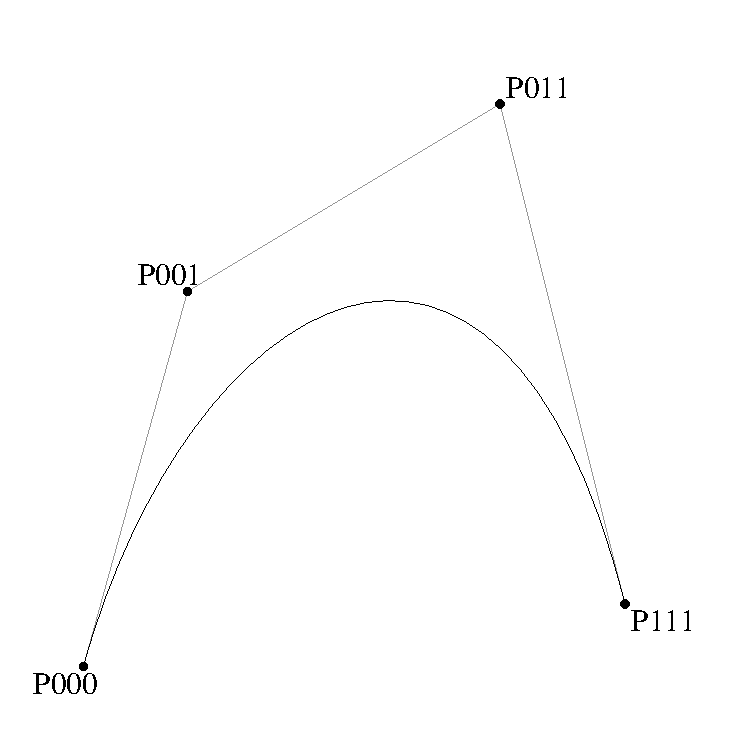
\includegraphics[height=4.5cm]{Ressources/pdf/f1.pdf}
    \end{center}

  \item
    Courbes paramétrées

     \medskip
    {\tiny
      $
      P000 = \begin{pmatrix}x_0\\y_0\end{pmatrix} \quad
        P001 = \begin{pmatrix}x_1\\y_1\end{pmatrix} \quad
          P011 = \begin{pmatrix}x_2\\y_2\end{pmatrix} \quad 
            P111 = \begin{pmatrix}x_3\\y_3\end{pmatrix}
              $
    }

    {\scriptsize
    \[
    \begin{cases}
    x(t) = x_0 (1-t)^3 + 3 x_1 (1-t)^2 t + 3 x_2 (1-t) t^2 + x_3 t^3 \\
    y(t) = y_0 (1-t)^3 + 3 y_1 (1-t)^2 t + 3 y_2 (1-t) t^2 + y_3 t^3
    \end{cases}
    \]
    }

  \end{itemize}
  
\end{frame}

\begin{frame}
  \frametitle{Propriétés}

  \begin{itemize}

  \item
    Une courbe de Bézier est incluse dans l'enveloppe convexe de ses points de contrôle (barycentres à poids positifs)

  \item
    Elle est tangente aux droites passant par les points de contrôle centraux et aux extrémités

  \item
    Pour effectuer une transformation affine sur une courbe de Bézier, il suffit de l'appliquer à ses points de contrôle
    
  \end{itemize}
  
\end{frame}

\begin{frame}
  \frametitle{\small Utilisation dans les description de glyphes}
  
  \begin{tabular}{ccc}
    \includegraphics[height=6.5cm]{Ressources/pdf/b1.pdf} &
    \includegraphics[height=6.5cm]{Ressources/pdf/b2.pdf} \\
                    {\scriptsize Décomposition en sous-courbes} & {\scriptsize Points de contrôle} \\
  \end{tabular}
\end{frame}

\subsection{Algorithme de De Casteljau}

\begin{frame}
  
  \begin{center}
    \begin{tabular}{cc}
      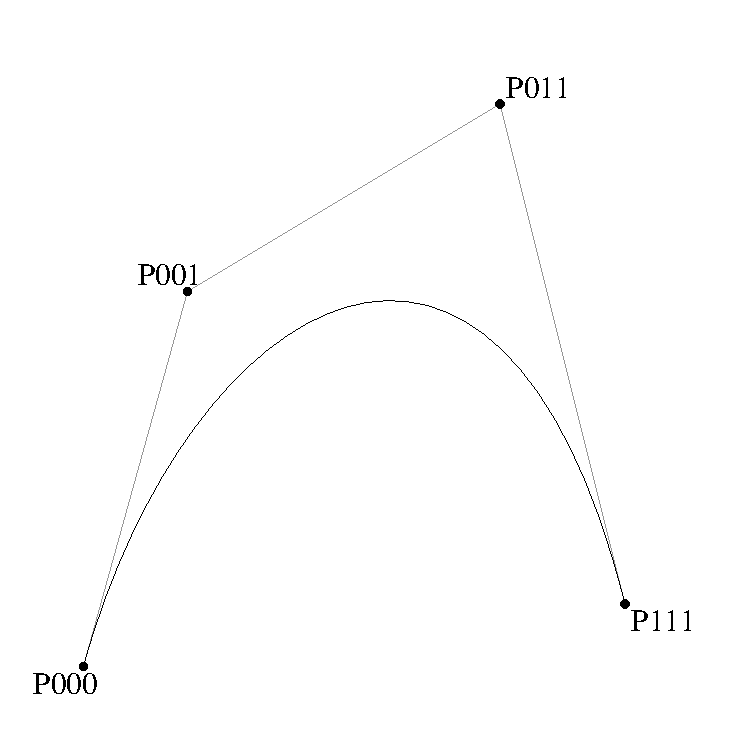
\includegraphics[height=4.2cm]{Ressources/pdf/f1.pdf} &
      \includegraphics[height=4.2cm]{Ressources/pdf/f2.pdf} \\
      \includegraphics[height=4.2cm]{Ressources/pdf/f3.pdf} & 
      \includegraphics[height=4.2cm]{Ressources/pdf/f4.pdf} \\
    \end{tabular}
  \end{center}
  
\end{frame}

\begin{frame}
  \frametitle{Principe}

  \begin{itemize}

  \item
    Algorithme récursif, basé sur la méthode « diviser pour régner »

  \item
    Les points de contrôle intermédiaires calculés par l'algorithme de De Casteljau décrivent les deux sous-courbes de part et d'autre du point $P_{ttt}$

    \item
      À chaque appel, on renvoie deux quadruplets de points de contrôle, construits par calculs successifs de barycentres. La moitié, ceux aux extrémités, sont des points de la courbe. Un appel est réalisé sur chacune des deux sous-courbes

  \end{itemize}
  
\end{frame}

\begin{frame}
  \frametitle{Preuve de correction}

  {\small
    \begin{itemize}
      
    \item
      Montrons que $P_{ttt} \in \mathcal{B}(P_{000},P_{001},P_{011},P_{111})$
      
      \begin{align*}
        P_{ttt}
        & = \bary \begin{pmatrix} P_{0tt} & P_{tt1} \\ t & 1-t\end{pmatrix} \\
          & = \bary \begin{pmatrix} P_{00t} & P_{0t1} & P_{t11} \\ t^2 & 2t(1-t) & (1-t)^2\end{pmatrix} \\
            & = \bary \begin{pmatrix} P_{000} & P_{001} & P_{011} & P_{111} \\ t^3 & 3t^2(1-t) & 3t(1-t)^2 & (1-t)^3\end{pmatrix}
      \end{align*}
      
    \end{itemize}
  }
  
\end{frame}

\begin{frame}
  \frametitle{Preuve de correction}

  {\small
    \begin{itemize}
      
    \item
      Montrons que $\mathcal{B}(P_{ttt},P_{tt1},P_{t11},P_{111}) \subset \mathcal{B}(P_{000},P_{001},P_{011},P_{111})$

      \medskip

      Soit \quad $P_{ppp} = \bary \begin{pmatrix} P_{000} & P_{00t} & P_{0t1} & P_{ttt} \\ p^3 & 3p^2(1-p) & 3p(1-p)^2 & (1-p)^3\end{pmatrix}$
        
        \medskip
      
        On montre que \quad $P_{ppp} = \bary \begin{pmatrix} P_{000} & P_{001} & P_{011} & P_{111} \\ \lambda^3 & 3\lambda^2(1-\lambda) & 3\lambda(1-\lambda)^2 & (1-\lambda)^3\end{pmatrix}$ \quad {\scriptsize où $\lambda = pt$}

        \item
          De même pour $\mathcal{B}(P_{000},P_{00t},P_{0tt},P_{ttt})$, avec $\mu$ tel que $1-\mu = (1-t)(1-p)$
          
    \end{itemize}
  }
  
\end{frame}

\section{PostScript Type 1}

\begin{frame}
  \center \LARGE \thesection. PostScript Type 1
\end{frame}

\lstset{language=PostScript,morekeywords={hmoveto,vlineto,rrcurveto,endchar,hsbw},basicstyle=\scriptsize,frame=single,captionpos=b}
\begin{frame}[fragile]

  \begin{itemize}

  \item
    Un fichier de fonte au format \emph{pfb} est converti au format \emph{asm}. On isole manuellement les descriptions des glyphes pour les lire avec Caml Light

  \item
    Format vectoriel : présence d'instructions de tracé plutôt que d'un bitmap

  \item
    Les fontes de Type 1 sont décrites dans le langage PostScript. La syntaxe est postfixée
    
    \begin{lstlisting}[title={\tiny \fbox{Extrait de la description du glyphe de \emph{b} en Arial}}]
      /b {
        134 1139 hsbw
        167 hmoveto
        133 vlineto
        71 -105 99 -52 125 0 rrcurveto
        126 0 108 50 90 99 rrcurveto
        ...
        closepath
        endchar
      } ND
    \end{lstlisting}
    
  \end{itemize}

\end{frame}

\section{Formule de Green-Riemann}

\begin{frame}
  \center \LARGE \thesection. Formule de Green-Riemann
\end{frame}

\begin{frame}
  \frametitle{Énoncé}

  Soit $\mathcal{C}$ un contour fermé du plan, \\
  décrit par une courbe paramétrée $(x,y)$.

  Alors l'aire de la portion de plan enclose par $\mathcal{C}$ est :

  \[\mathcal{A} = \frac{1}{2} \int_{\mathcal{C}} (x \mathrm{d}y - y \mathrm{d}x)\]
  
\end{frame}

\begin{frame}
  \frametitle{Démonstration}
  \framesubtitle{Lemme}

  Soit ABDC un parallélogramme. Alors
  \[\mathcal{A}_{ABDC} = \det{(\overrightarrow{AB},\overrightarrow{AC})}
  \qquad \mathcal{A}_{ABC} = \frac{1}{2} \det{(\overrightarrow{AB},\overrightarrow{AC})}\]

  \begin{center}
    \begin{tikzpicture}[line cap=round,line join=round,>=triangle 45,x=10mm,y=10mm]
      \clip(-0.31,-0.29) rectangle (4.19,2.36);
      \fill[line width=0.4pt,fill=black,fill opacity=0.15] (0,0) -- (3,0) -- (4,2) -- (1,2) -- cycle;
      \draw (0,0)-- (3,0);
      \draw (0,0)-- (1,2);
      \draw (1,2)-- (4,2);
      \draw (3,0)-- (4,2);
      \draw [line width=0.4pt] (0,0)-- (3,0);
      \draw [line width=0.4pt] (3,0)-- (4,2);
      \draw [line width=0.4pt] (4,2)-- (1,2);
      \draw [line width=0.4pt] (1,2)-- (0,0);
      \draw [dash pattern=on 1pt off 1pt] (1,2)-- (1,0);
      \draw [dash pattern=on 1pt off 1pt] (3,2)-- (3,0);
      \begin{scriptsize}
        \fill [color=black] (0,0) circle (1.5pt);
        \draw[color=black] (0,-0.19) node {$A$};
        \fill [color=black] (3,0) circle (1.5pt);
        \draw[color=black] (3.04,-0.19) node {$B$};
        \fill [color=black] (1,2) circle (1.5pt);
        \draw[color=black] (0.99,2.23) node {$C$};
        \fill [color=black] (4,2) circle (1.5pt);
        \draw[color=black] (4.03,2.19) node {$D$};
        \fill [color=black] (1,0) circle (1.5pt);
        \draw[color=black] (1.02,-0.19) node {$H$};
        \fill [color=black] (3,2) circle (1.5pt);
        \draw[color=black] (3.02,2.24) node {$H'$};
      \end{scriptsize}
    \end{tikzpicture}
  \end{center}
  
\end{frame}

%\begin{frame}
%  \frametitle{Démonstration}
%  \framesubtitle{Rappel}
%  
%  \textbf{Démonstration de la propriété}
%  
%  Notons $H$ le projeté orthogonal de $C$ sur $[AB]$. On a alors
%  \begin{align*}
%    & \det{(\overrightarrow{AB},\overrightarrow{AC})} \\
%    = & \det{(\overrightarrow{AH}+\overrightarrow{HB},\overrightarrow{AH}+\overrightarrow{HC})} \\
%    = & \det{(\overrightarrow{HC},\overrightarrow{AH})} + \det{(\overrightarrow{HC},\overrightarrow{HB})} \\
%    = & AH \cdot HC + HB \cdot HC \\
%    = & \mathcal{A}_{ABDC} \\
%  \end{align*}
%
%  D'où $\mathcal{A}_{ABC} = \frac{1}{2} \det{(\overrightarrow{AB},\overrightarrow{AC})}$.
%  
%\end{frame}

\begin{frame}
  \frametitle{Démonstration}
  
  \begin{figure}
    \includegraphics[width=7.5cm]{Ressources/Images/Green-Riemann2.png}
  \end{figure}
  
\end{frame}

\begin{frame}
  \frametitle{Démonstration}

  \textbf{Démonstration de la formule de Green-Riemann}
  
  On a $\mathrm{d}x = \dot x(t) \mathrm{d}t$ et $\mathrm{d}y = \dot y(t) \mathrm{d}t$, donc
  \begin{align*}
    \frac{1}{2} \int_{\mathcal{C}}(x \mathrm{d}y - y \mathrm{d}x)
    = & \frac{1}{2} \int_{\mathcal{C}}(x \dot y - y \dot x) \mathrm{d}t \\
    = & \frac{1}{2} \int_{\mathcal{C}}
    \begin{vmatrix}
      x & \dot x \\
      y & \dot y
    \end{vmatrix} \mathrm{d}t \\
    = & \frac{1}{2} \int_{\mathcal{C}} \det(\overrightarrow{OM},\overrightarrow{v}) \mathrm{d}t \\
    = & \int_{\mathcal{C}} \frac{1}{2} \det(\overrightarrow{OM},\overrightarrow{v} \mathrm{d}t) \\
    = & \int_{\mathcal{C}} \mathrm{d}S \\
    = & \mathcal{A}
  \end{align*}
  
\end{frame}

\section{Résultats}

\begin{frame}
  \center \LARGE \thesection. Résultats
\end{frame}

\subsection{Méthode de calcul}

\begin{frame}

  \begin{itemize}

  \item
    Calcul des hauteurs des glyphes des caractères par construction de la bounding box

    \begin{center}
      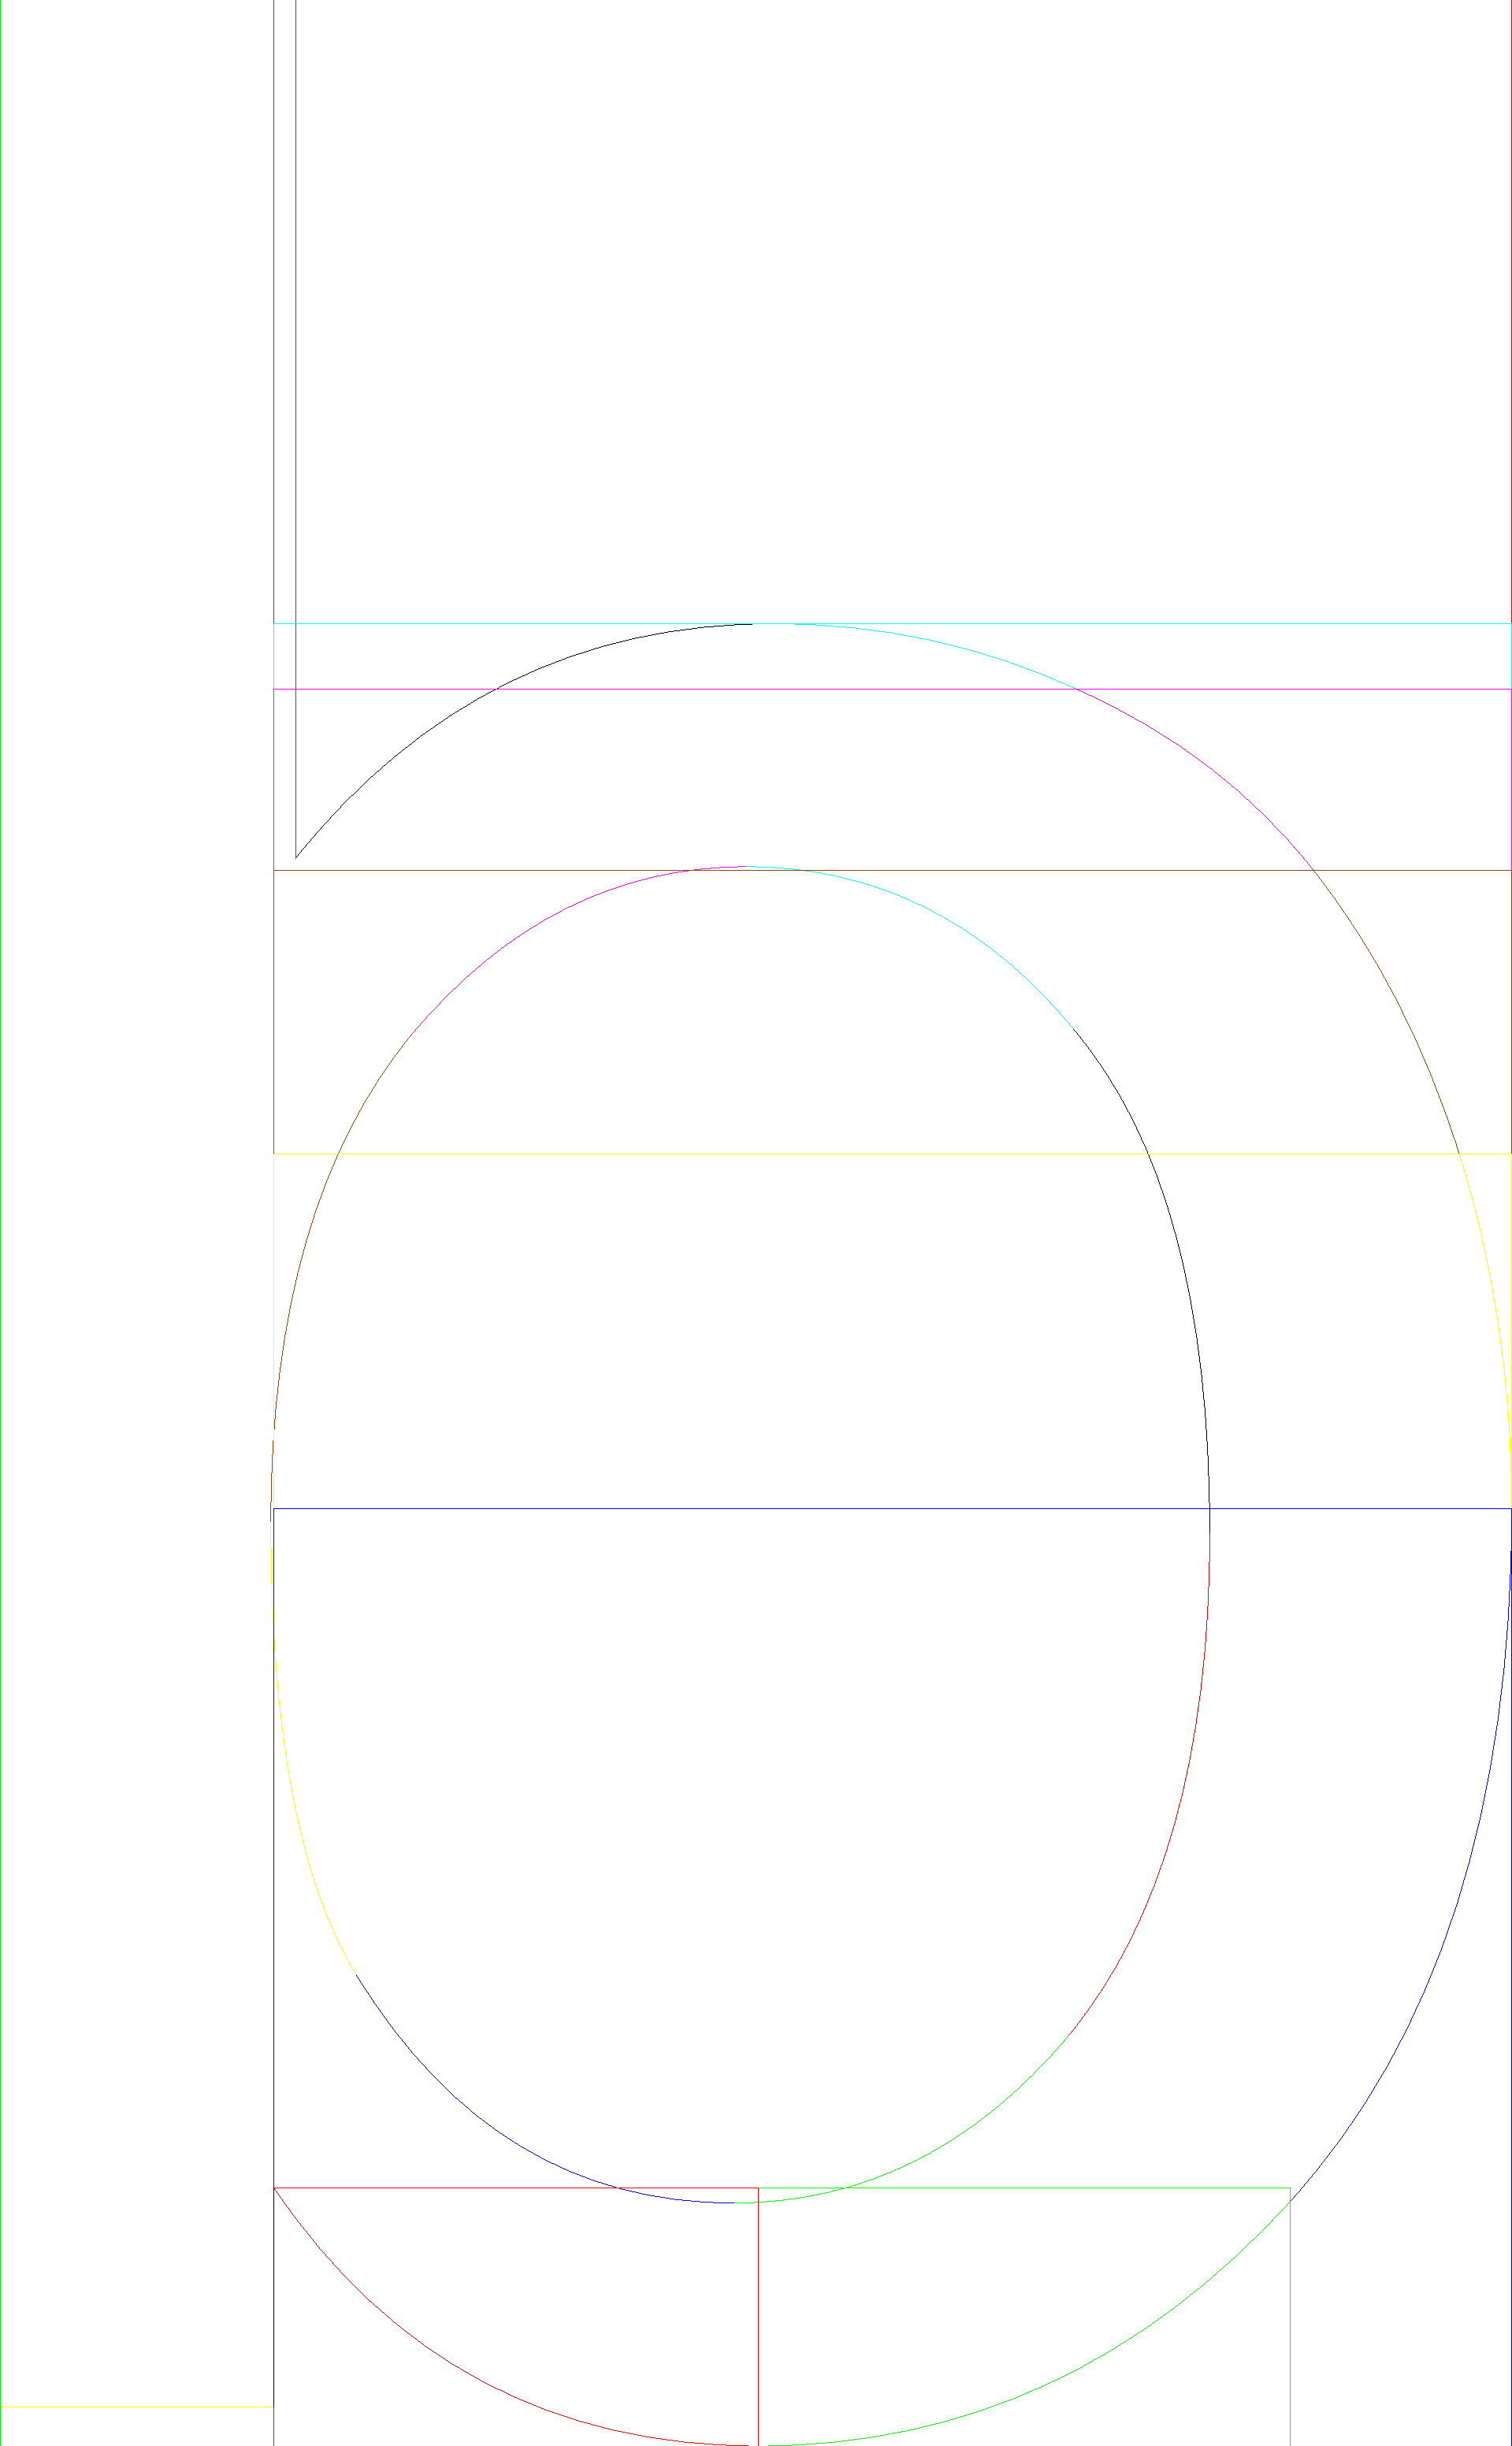
\includegraphics[height=6cm]{Ressources/pdf/b3.pdf}
    \end{center}
    
  \item  
    Les aires des sections du glyphes sont sommées au fur et à mesure du parcours de ce dernier

    %Suivi graphique
    
  \end{itemize}
  
\end{frame}

\subsection{Résultats}

\begin{frame}
  \frametitle{Fréquences d'apparition}

  {\small
  \begin{tabular}{c|c|c}
    \diagbox{Lettre}{\OE uvre} & La Bête Humaine & Thèse L. de Broglie \\
    \hline \\
    e & 15.9 \%& 16.2 \% \\
    \hline \\
    a & 8.68 \% & 6.26 \% \\
    \hline \\
    i & 7.08 \% & 6.37 \% \\
    \hline \\
    t & 7.04 \% & 6.93 \% \\
    \hline \\
    s & 6.98 \% & 7.32 \% \\
    \hline \\
    r & 6.23 \% & 5.92 \% \\
    \hline \\
    o & 4.55 \% & 6.03 \% \\
  \end{tabular}
  }
  
\end{frame}

\begin{frame}
  \frametitle{Aires pondérées relatives}

  {\small
  \begin{tabular}{c||c|c|c}
    Hauteur d'x & \diagbox{Fonte}{\OE uvre} & L.B.H. & Thèse\\
    \hline \\
    1062 & Arial & 0.377 & 0.399 \\
    \hline \\
    1120 & DejaVu Sans & 0.364 & 0.385 \\
    \hline \\
    916 & Times & 0.363 & 0.386 \\
    \hline \\
    409 & Garamond & 0.356 & 0.370 \\
    \hline \\
    1149 & Comic Sans MS & 0.351 & 0.374 \\
    \hline \\
    866 & Courier New & 0.320 & 0.330 \\
  \end{tabular}
  }
  
\end{frame}

\begin{frame}
  \frametitle{Critique}

  \begin{itemize}

  \item
    La fréquence d'apparition des caractères diffère significativement d'un document à l'autre, d'un type de document à un autre

  \item
    La fonte Garamond ne se démarque pas particulièrement des autres fontes en terme d'économies d'encre. Il vaut mieux privilégier l'esthétique, et surtout la lisibilité

  \item
    D'autres paramètres sont à prendre en compte, comme la consommation de papier ou l'entretien d'une imprimante, et rendent moindres les bénéfices liés à un choix de fonte particulier

  \end{itemize}
  
\end{frame}

\end{document}
